\documentclass[preprint,12pt]{elsarticle}

    \usepackage[sc]{mathpazo} % Use the Palatino font
    \usepackage[T1]{fontenc} % Use 8-bit encoding that has 256 glyphs
    \usepackage{microtype} % Slightly tweak font spacing for aesthetics
    \usepackage[english]{babel} % Language hyphenation and typographical rules
    \usepackage{booktabs} % Horizontal rules in tables
    \usepackage{enumitem} % Customized lists
    \usepackage[table,xcdraw]{xcolor}
    \usepackage[utf8]{inputenc} % Required for inputting international characters
    \usepackage{parskip}
    \usepackage{graphicx}
    \usepackage{hyperref}
    \usepackage{pdfpages}
    \usepackage{amsmath}
    \usepackage{esvect}
    \usepackage{listings}
    \usepackage{color}
    \usepackage{spverbatim}
    \usepackage{subcaption}
    \usepackage[title]{appendix}
    \hypersetup{
        colorlinks=true,
        linkcolor=blue,
        filecolor=magenta,      
        urlcolor=cyan,
    }
    \definecolor{dkgreen}{rgb}{0,0.6,0}
    \definecolor{gray}{rgb}{0.5,0.5,0.5}
    \definecolor{mauve}{rgb}{0.58,0,0.82}
    \definecolor{lightgray}{rgb}{0.83, 0.83, 0.83}
    \definecolor{timberwolf}{rgb}{0.86, 0.84, 0.82}
    \definecolor{whitesmoke}{rgb}{0.96, 0.96, 0.96}
    
    \lstset{frame=tb,
    language=python,
    aboveskip=3mm,
    belowskip=3mm,
    showstringspaces=false,
    columns=flexible,
    basicstyle={\small\ttfamily},
    numbers=none,
    numberstyle=\tiny\color{gray},
    keywordstyle=\color{blue},
    commentstyle=\color{dkgreen},
    stringstyle=\color{mauve},
    breaklines=true,
    breakatwhitespace=true,
    tabsize=3,
    backgroundcolor = \color{whitesmoke}
    }

    \begin{document}
    \title{\LARGE \bf
        STAT 391 Homework 4
        }
        
        \author{ \parbox{3 in}{\centering Chongyi Xu \\
                 University of Washington\\
                 STAT 391 Spring 2018\\
                 {\tt\small chongyix@uw.edu}}
        }
    \maketitle

    \section{Problem 1 - Rescuing Rob}
    \begin{enumerate}
        \item Estimate the parameters $\mu$ and $\sigma^2$ of the 
        normal density that best fits the data in the file hw4-ugrad.dat
        by the Maximum Likelihood method.\\

        The Maximum Likelihood estimation basiclly calculate for 
        the mean and the variance of the given data $\mathbb{X}$ and 
        use the sample mean as $\mu$ and the sample variance as $\sigma^2$

        \begin{lstlisting}
from statistics import *

# Read in files
# a) hw4-ugrad.dat
dir = r'C:\Users\johnn\Documents\UW\SchoolWorks\2018Spring\STAT391\HW4'
f = open(dir+r'\hw4-ugrad.dat')

x = [float(xx) for xx in f.readline().split(' ')]

# ML mu is the mean of data
mu = mean(x)

# ML sigma is the variance of the data
sigma = stdev(x)

print('The estimated mu is ', mu)
print('And the estimated sigma^2 is ', sigma**2)
        \end{lstlisting}

        And the result I got is 
        \begin{spverbatim}
The estimated mu is  10.018379536
And the estimated sigma^2 is  1.029920746065191
        \end{spverbatim}

        \item Estimate the parameters $a,b$ of the logistic density
        that best fits the data in the file hw4-boiler.dat by the
        Maximum Likelihood method. Make a plot of the log-likelihood
        of the data at each iteration.\\

        From lecture notes (6.24), we obtained the log-likelihood
        of the logistic density distribution,

        \begin{equation*}
            l(a,b) = nln(a) - a\sum_{i}x_i - nb - 2\sum_{i} ln(1+e^{-ax_i-b})
        \end{equation*}

        And therefore, the partial derivatives with respecting to $a,b$  are
        \begin{align*}
            \frac{\partial l}{\partial a} &= \frac{n}{a} - \sum_{i} x_i\frac{1-e^{-ax_i-b}}{1+e^{-ax_i-b}}\\
            \frac{\partial l}{\partial b} &= -\sum_{i} \frac{1-e^{-ax_i-b}}{1+e^{-ax_i-b}}
        \end{align*}

        Since the system is not able to solved analytically, we have to guess for the 
        solution by gradient ascent. The estimated $\hat{a},\hat{b}$ are 
        \begin{align*}
            \hat{a} &\leftarrow \tilde{a} + \eta \frac{\partial l}{\partial a}\\
            \hat{b} &\leftarrow \tilde{b} + \eta \frac{\partial l}{\partial b}
        \end{align*}
        where $\tilde{a}=1$ and $\tilde{b}=0$ are the intial guess for $a,b$.

        \begin{lstlisting}
import numpy as np
import math
import matplotlib.pyplot as plt

dir = r'C:\Users\johnn\Documents\UW\SchoolWorks\2018Spring\STAT391\HW4'
f = open(dir+r'\hw4-boiler.dat')

x = [float(xx) for xx in f.readline().split(' ')]

step = 0.00001
n = len(x)
iterations = 5000
ll = [0.0]*iterations
a = [0.0]*iterations
b = [0.0]*iterations
a[0] = 1

for i in range(iterations):
ll[i] = n * math.log(a[i]) - n * b[i]
dlda = n / a[i]
dldb = 0
for xi in x:
    ll[i] += - a[i] * xi - 2 * math.log(1 + \
                math.exp(-a[i] * xi - b[i]))
    dlda -= xi * (1 - math.exp(-a[i] * xi - b[i]))\
                /(1 + math.exp(-a[i] * xi - b[i]))
    dldb -= (1 - math.exp(-a[i] * xi - b[i]))\
                /(1 + math.exp(-a[i] * xi - b[i]))
if i + 1 < iterations:
    a[i+1] = a[i] + step * dlda
    b[i+1] = b[i] + step * dldb

plt.figure(1)
plt.plot(np.arange(iterations), ll)
plt.title('Log-likelihood')
plt.xlabel('Iteration')
plt.show()

plt.figure(2)
plt.plot(a,b, 'o', Linewidth=0.8)
plt.title('Parameters a,b')
plt.xlabel('a')
plt.ylabel('b')
plt.show()
        \end{lstlisting}

        \begin{figure}[htbp!]
            \center
            \begin{subfigure}{0.8\textwidth}
                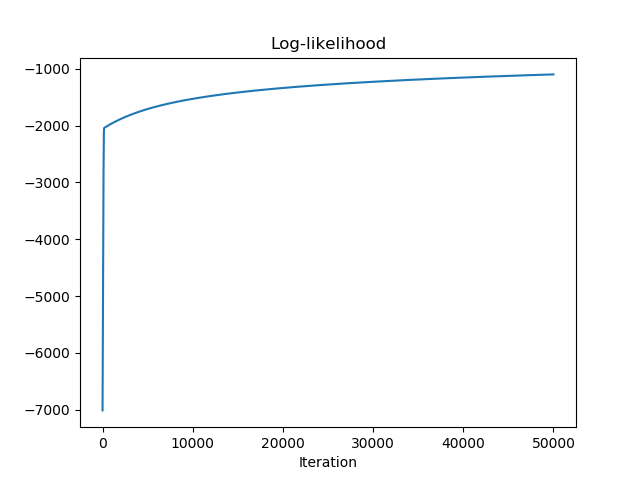
\includegraphics[width = \textwidth]{1.png}
                \caption{The Log-likelihood of the data}
                \label{fig:11}
            \end{subfigure}
            \begin{subfigure}{0.8\textwidth}
                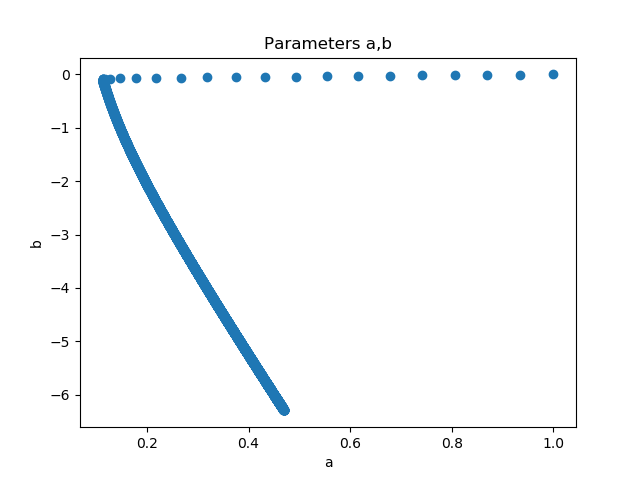
\includegraphics[width = \textwidth]{2.png}
                \caption{The values of paramter $a,b$}
                \label{fig:12}
            \end{subfigure}
            \caption{Estimation of logistic density}
            \label{fig:1}
        \end{figure}
        And the plot is Figure \ref{fig:1}.\\

        And since we are expecting the Maximum Likelihood estimation of 
        $\hat{a},\hat{b}$ are $arg max ll(x;a,b)$. And the iteration method
        will be guaranteed to converge to a local maximum of the log-likelihood,
        therefore, the $a,b$ are
        \begin{lstlisting}
i,=np.where(np.array(ll)==max(ll))
a_ML = a[i[0]]
b_ML = b[i[0]]
print('The estimated a is ', a_ML)
print('The estimated b is ', b_ML)
        \end{lstlisting}

        \begin{spverbatim}
The estimated a is  0.4699146245081937
The estimated b is  -6.2957753505203815    
        \end{spverbatim}

        \item Compute a kernel density estimate for the data in the file
        hw4-coke.dat using a Gaussian kernel with kernel width $h=0.5$.\\

        Since we are using a Gaussian kernel, then
        \begin{align*}
            k(x) &= \frac{1}{\sqrt{2\pi}}e^{-\frac{x^2}{2}}\\
            \Rightarrow f_X(x) &= \frac{1}{nh}\sum_{i=1}^n k(\frac{x-x_i}{h}) \\
            &= \frac{1}{500\cdot 0.5}\sum_{i} \frac{1}{\sqrt{2\pi}} exp(\frac{(-\frac{x-x_i}{h})^2}{2})\\
            &= \frac{1}{250\sqrt{2\pi}}\sum_{i} e^{-2(x-x_i)^2}
        \end{align*}

        \item After having had his memory restored, Rob suddenly finds himself
        facing an unknown object whose signature is given in the file hw4-unknown.dat.
        Help Rob once more: tell him what is the object in front of him.\\

        Find log-likelihood for each type.
        \begin{align*}
            ll_{people}(x_{test}; \mu,\sigma^2) &= -\frac{n}{2}ln(2\pi) - \frac{n}{2}ln(\sigma^2) - \frac{1}{2\sigma^2}\sum_{i} (x_i - \mu)^2 \\
            ll_{furniture}(x_{test};a,b) &= nln(a) - a\sum_{i}x_i - nb - 2\sum_{i} ln(1+e^{-ax_i-b}) \\
            ll_{trash}(x_{test};x_{train}) &= \frac{1}{250\sqrt{2\pi}}\sum_{i} e^{-2(x-x_i)^2}
        \end{align*}



    \end{enumerate}

    \section{Problem 2 - Maximum Likelihood with censored data}
\end{document}